\documentclass[a4paper,12pt]{article} % тип документа

%  Русский язык
\usepackage[T2A]{fontenc}			% кодировка
\usepackage[utf8]{inputenc}			% кодировка исходного текста
\usepackage[english,russian]{babel}	% локализация и переносы

\usepackage{graphicx}               % импорт изображений
\usepackage{wrapfig}                % обтекаемые изображения
\graphicspath{{pictures/}}          % обращение к подкаталогу с изображениями
\usepackage[14pt]{extsizes}         % для того чтобы задать нестандартный 14-ый размер шрифта
\usepackage{amsfonts}               % буквы с двойными штрихами
\usepackage[warn]{mathtext}         % русский язык в формулах
\usepackage{indentfirst}            % indent first
\usepackage[margin = 25mm]{geometry}% отступы полей
\usepackage{amsmath}                % можно выводить фигурные скобочки -- делать системы уравнений
\usepackage[table,xcdraw]{xcolor}   % таблицы
\usepackage{amsmath,amsfonts,amssymb,amsthm,mathtools} % Математика
\usepackage{wasysym}                % ???
\usepackage{upgreek}                % ???  
\usepackage{caption}
\captionsetup{labelsep=period}
\usepackage{gensymb} % degree symbol
\usepackage{mathrsfs}
\usepackage{multirow}

\begin{document}
	\begin{center}
		
		\textbf{НАЦИОНАЛЬНЫЙ ИССЛЕДОВАТЕЛЬСКИЙ УНИВЕРСИТЕТ \\ <<МОСКОВСКИЙ ФИЗИКО-ТЕХНИЧЕСКИЙ ИНСТИТУТ>>}
		\vspace{13ex}
		
		\textbf{Лабораторная работа 3.3.4 \\ <<Эффект Холла в полупроводниках>> }
		\vspace{60ex}
		
		\normalsize{Овсянников Михаил Александрович \\ студент группы Б01-001\\ 2 курс ФРКТ\\}
	\end{center}
	
	\vfill 
	
	\begin{center}
		г. Долгопрудный\\ 
		2021 г.
	\end{center}
	
	\thispagestyle{empty} % выключаем отображение номера для этой страницы
	
	\newpage
	
\textbf{Цель работы:} изучить эффект Холла, определить концентрацию и подвижность заряженных частиц в образце германия.

\vspace{5mm}
\textbf{В работе используются:} электромагнит с источником питания GPR, батарейка 1,5 В, амперметр, реостат, цифровой вольтметр В7-78/1, милливеберметр, образцы легированного германия.

\vspace{7mm}
\textbf{Экспериментальная установка.} 

\begin{figure}[h!]
	\centering
	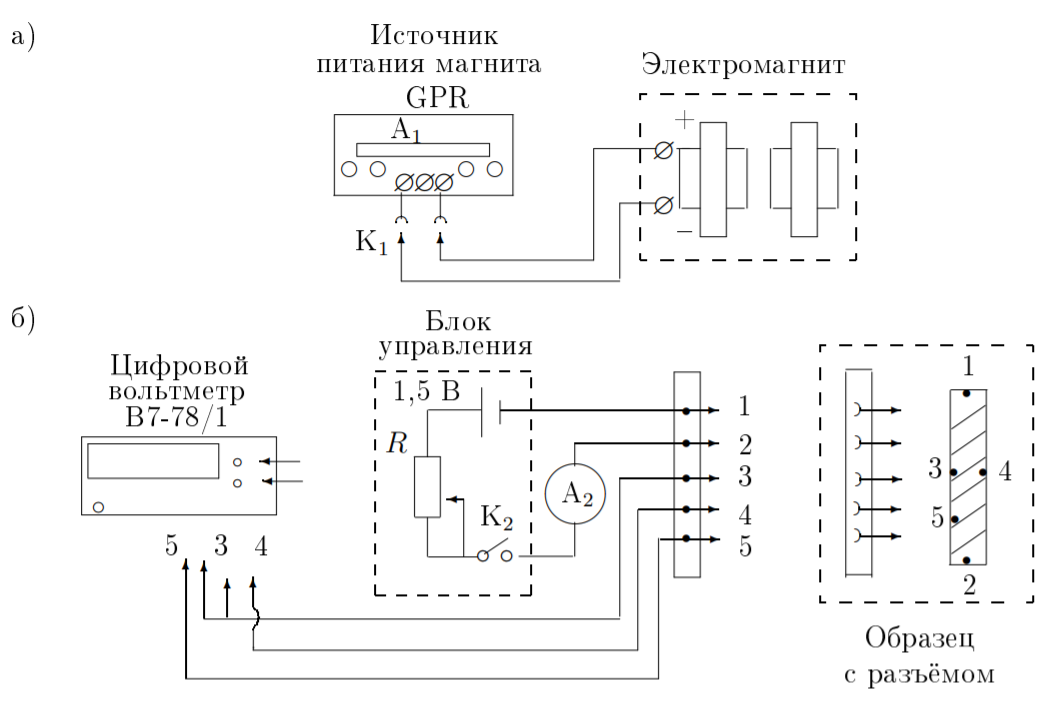
\includegraphics[scale=0.7]{Pictures/Установка.png}
	\caption*{Рис. 1. Схема установки для исследования эффекта Холла}
\end{figure}

В зазоре электромагнита (Рис. 1а) создается постоянное магнитное поле, величину которого можно менять с помощью регуляторов источника питания.

Образец легированного германия, смонтированный в специальном держателе (Рис. 1б), подключается к батарее ($\approx$ 1,5 В).

В образце с током, помещенном в зазор электромагнита, между контактами 3 и 4 возникает разность потенциалов $U_{34}$, которая измеряется с помощью цифрового вольтметра.

Контакты 3 и 4 вследствие неточности подпайки не всегда лежат на одной эквипотенциали, поэтому напряжение связано не только с эффектом Холла, но и омическим падением напряжения. Тогда измеряемая разность потенциалов в одном направлении магнитного поля равна сумме ЭДС Холла и омического падения напряжения, а в другом - их разности. 

Можно исключить омическое падение напряжения по-другому - при фиксированном значении тока $I$ оно является постоянным $U_0$. Тогда $\mathscr{E} = U_{34} \pm U_0$.

\vspace{10mm}

{\LARGE \textbf{Ход работы}}

\begin{figure}[h!]
	\centering
	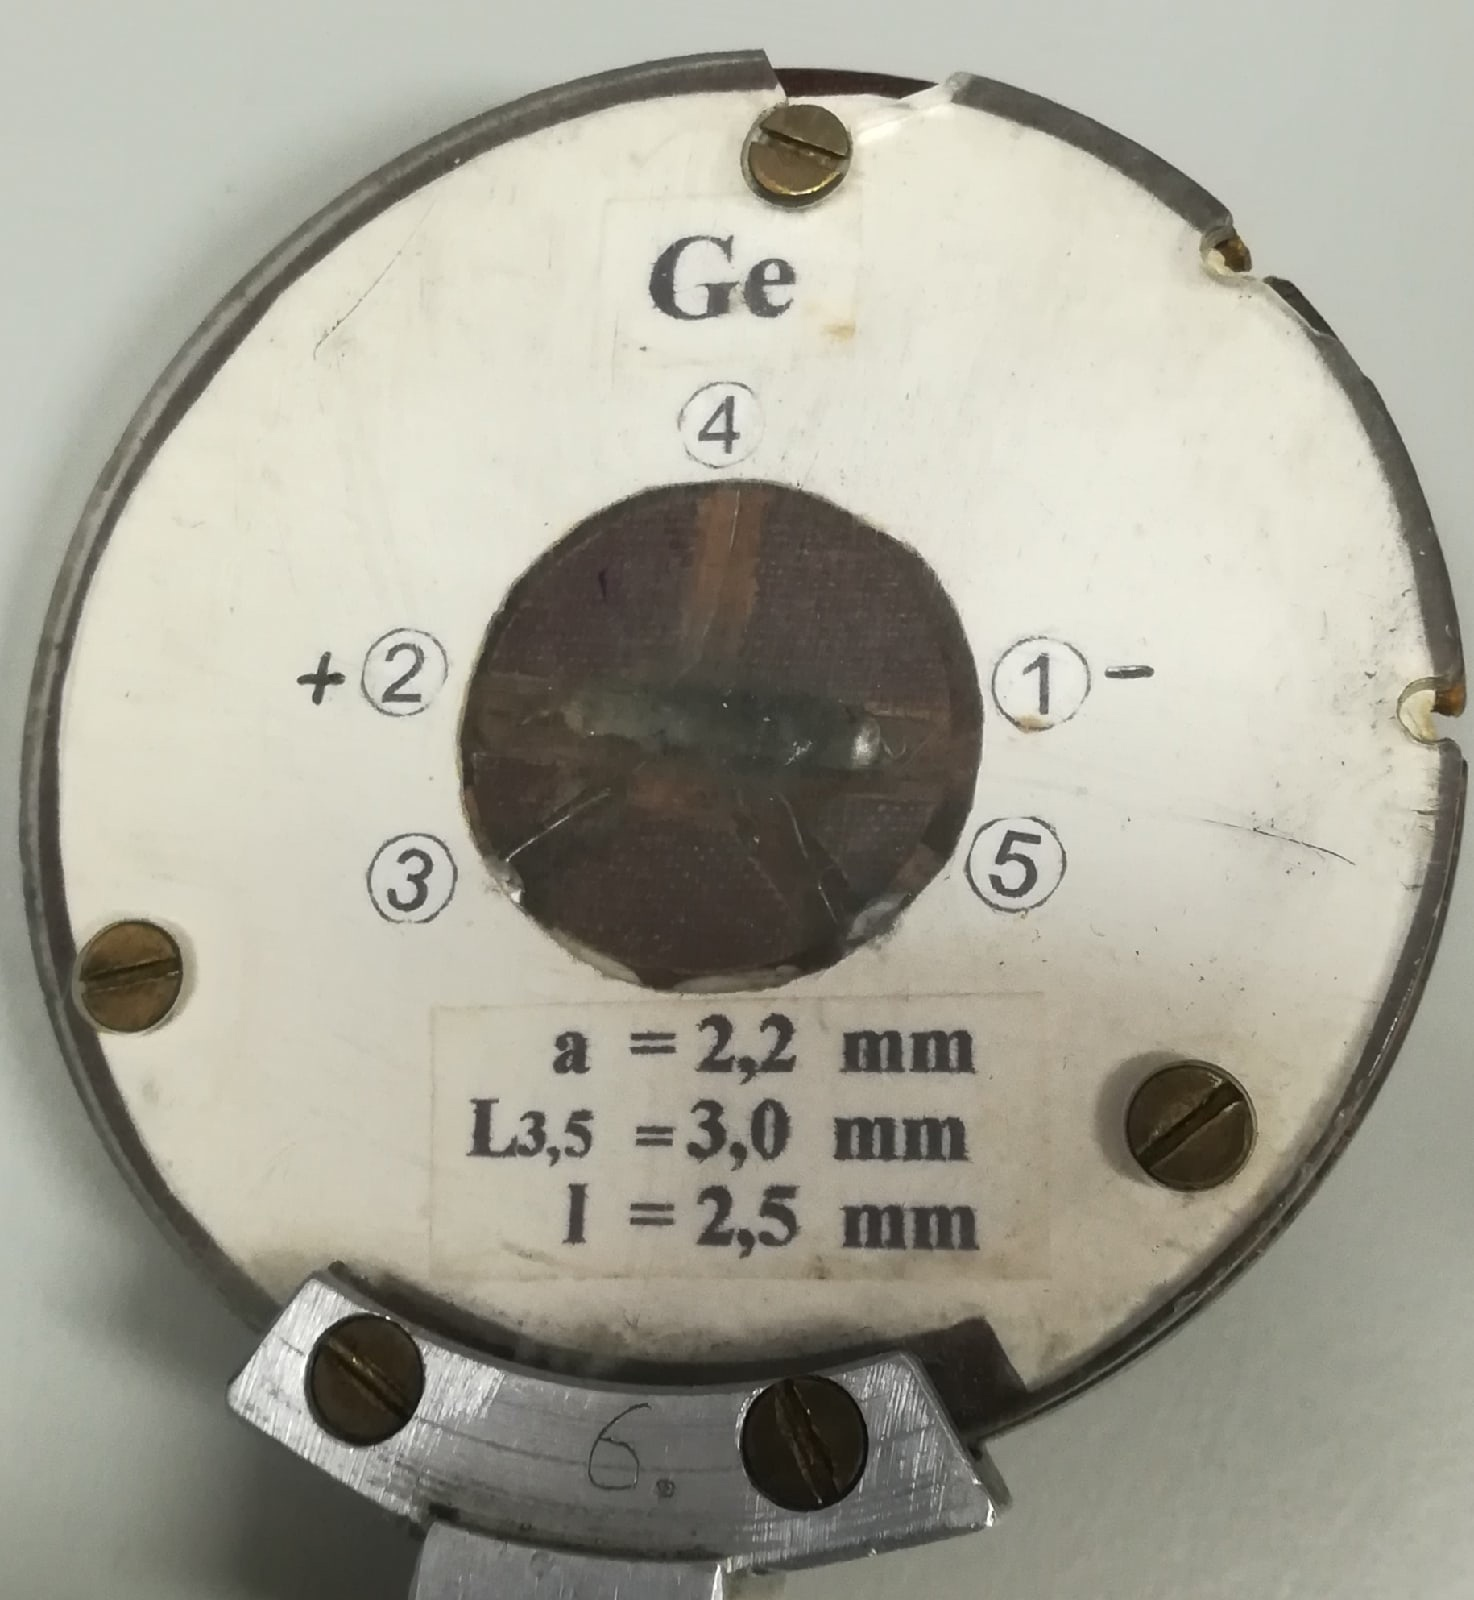
\includegraphics[scale=0.31]{Pictures/Образец.jpg}
	\caption*{Рис. 2. Образец}
\end{figure}

Зафиксируем параметры образца:

$a = 2,2$ мм - это ширина образца;

$L_{35} = 3,0$ мм - это расстояние между контактами;

$h = 2,5$ мм - это толщина образца.

\vspace{5mm}
Проведем градуировку электромагнита и запишем результаты в таблицу 1:

\begin{table}[h!]
	\centering
	\begin{tabular}{|c|c|c|c|c|c|c|c|c|c|}
		\hline
		$B$, мТл & 1057 & 1032 & 978 & 935 & 845 & 730 & 611 & 491 & 338 \\ \hline
		$I$, А   & 2,0  & 1,8  & 1,6 & 1,4 & 1,2 & 1,0 & 0,8 & 0,6 & 0,4 \\ \hline
	\end{tabular}
	\caption*{Таблица 1}
\end{table}

Снимем вольт-амперную характеристику образца. Запишем все измерения в таблицу 2:

\begin{table}[h!]
	\centering
	\begin{tabular}{|c|c|c|c|c|c|c|c|c|c|}
		\hline
		$I$, мА  & 0,2 & 0,3 & 0,4 & 0,5 & 0,6  & 0,7  & 0,8  & 0,9  & 1,0  \\ \hline
		$U$, мкВ & 361 & 530 & 703 & 875 & 1043 & 1220 & 1392 & 1565 & 1743 \\ \hline  
	\end{tabular}
	\caption*{Таблица 2}
\end{table}

Построим график $U(I)$:
\begin{figure}[h!]
	\centering
	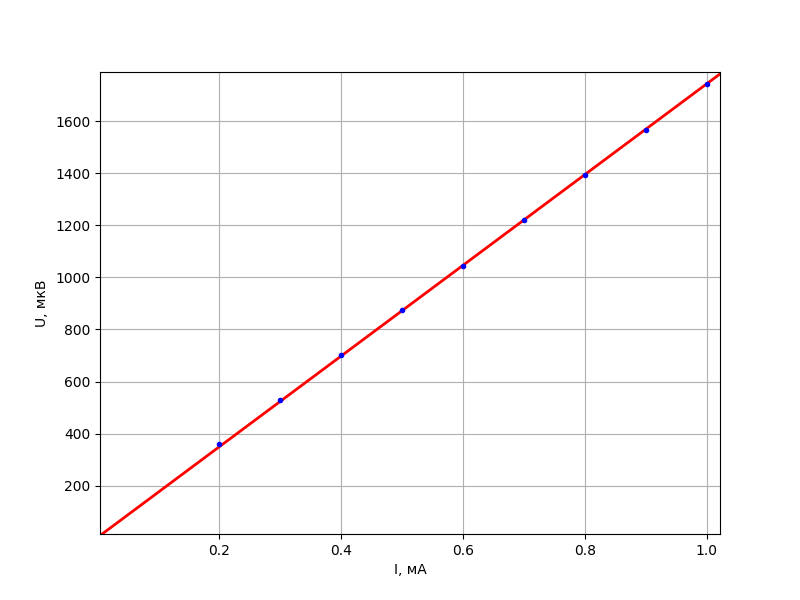
\includegraphics[scale=0.73]{Pictures/U(I).png}
	\caption*{Рис. 3.}
\end{figure}

Используя МНК:

$U(I) = R \cdot I$;

$R = 1,742$ Ом;

$\sigma_R = 0,002$ Ом.

\vspace{7mm}
Найдем удельное сопротивление $\rho_0$ образца германия:

$\rho_0 = R\frac{ah}{L_{35}} = 0,312$ Ом$\cdot$см.

$\sigma_{\rho_0} = \rho_0\cdot\frac{\sigma_R}{R} = 0,0004$ Ом$\cdot$см.

Итого: $\boxed{\rho_0 = (3120 \pm 4)\cdot 10^{-4} \text{ Ом}\cdot\text{см}}$

\vspace{7mm}

Теперь найдем удельную проводимость $\sigma = \frac{1}{\rho_0} = 3,2$ (Ом$\cdot$см)$^{-1}$.

Ее погрешность $\sigma_{\sigma} = \sigma \cdot \frac{\sigma_{\rho_0}}{\rho_0} = 0,004$ (Ом$\cdot$см)$^{-1}$.

Итого: $\boxed{\sigma = (3,200 \pm 0,004) \text{ } (\text{Ом}\cdot\text{см})^{-1}}$

\vspace{12mm}
Исследуем зависимость ЭДС Холла от магнитного поля магнита при различных значениях продольного тока. Примем во внимание тот факт, что напряжение на контактах также связано с омическим падением напряжения, поэтому можно найти само ЭДС Холла двумя путями:

$1) U_{\text{ср}} = \frac{(+U_X) -( -U_X)}{2} \hspace{70mm} 2)U_{\text{ср}} = U_{34} - U_0$ 

\vspace{7mm}
{\Large \textbf{1.}} $I_0 = 1$ мА, $U_0 = -38$ мкВ.


\begin{table}[h!]
	\centering
	\begin{tabular}{|c|c|c|c|c|c|}
		\hline
		\multirow{2}{*}{$I$, А} & \multirow{2}{*}{$B$, мТл} & \multirow{2}{*}{$+U_X$, мкВ} & \multirow{2}{*}{$-U_X$, мкВ} & \multicolumn{2}{c|}{$U_{\text{ср}}$}                   \\ \cline{5-6} 
		&                           &                              &                              & $\frac{(+U_X) - (-U_X)}{2}$, мкВ & $U_{34} - U_0$, мкВ \\ \hline
		2,0                     & 1057                      & 166                          & -237                         & 202                              & 204                 \\ \hline
		1,8                     & 1032                      & 157                          & -230                         & 194                              & 195                 \\ \hline
		1,6                     & 978                       & 149                          & -221                         & 185                              & 187                 \\ \hline
		1,4                     & 935                       & 137                          & -210                         & 174                              & 175                 \\ \hline
		1,2                     & 845                       & 121                          & -193                         & 157                              & 159                 \\ \hline
		1,0                     & 730                       & 99                           & -172                         & 136                              & 137                 \\ \hline
		0,8                     & 611                       & 75                           & -148                         & 112                              & 113                 \\ \hline
		0,6                     & 491                       & 49                           & -122                         & 86                               & 87                  \\ \hline
		0,4                     & 338                       & 23                           & -95                          & 59                               & 61                  \\ \hline
	\end{tabular}
	\caption*{Таблица 3}
\end{table}

Как видим, значения, полученные этими двумя способами, достаточно близки друг к другу.
\vspace{7mm}

Строим график $\mathscr{E}_X(B) = U_{\text{ср}}(B)$.

\begin{figure}[h!]
	\centering
	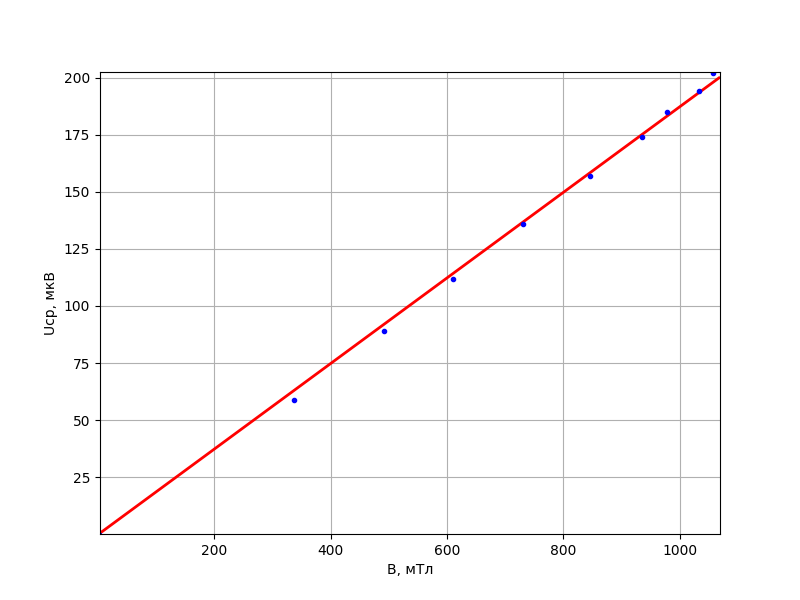
\includegraphics[scale=0.73]{Pictures/1мАмпер.png}
	\caption*{Рис. 4.}
\end{figure}

Используя МНК, получаем:

$\mathscr{E}_X = \frac{I_0B}{nea} = R_X\cdot\frac{I_0B}{a} = k_1B$.

$k_1 = 18,8 \cdot 10^{-5}$ $\frac{\text{В}}{\text{Тл}} = 18,8 \cdot 10^{-5}\text{ }\frac{\text{м}^2}{\text{c}}$ 

$\sigma_{k_1} = 0,1 \cdot 10^{-5}$ $\frac{\text{м}^2}{\text{c}}$.

Откуда получаем:
\vspace{2mm}

$n = \frac{I_0}{k_1ea} = 1,51\cdot 10^{16}$ см$^{-3}$; \hspace{42mm} $R_X = \frac{ak_1}{I_0} = 414\text{ }\frac{\text{см}^3}{\text{Кл}}$;

\vspace{2mm}
$\sigma_n = n\cdot \frac{\sigma_{k_1}}{k_1} = 0,01\cdot 10^{16}$ см$^{-3}$; \hspace{40mm} $\sigma_{R_X} = R_X \cdot \frac{\sigma_{k_1}}{k_1} = 2\text{ }\frac{\text{см}^3}{\text{Кл}}$;

\vspace{3mm}
$\boxed{n = (1,51 \pm 0,01)\cdot 10^{16} \text{ см}^{-3}} \hspace{38mm} \boxed{R_X = (414 \pm 2)\text{ }\frac{\text{см}^3}{\text{Кл}}}$

\vspace{7mm}
Найдем подвижность частиц $\mu$ из уравнения $\sigma = ne\mu$:

$\mu = \frac{\sigma}{ne} = 1,32\cdot 10^2$ $\frac{\text{см}^2}{\text{В}\cdot\text{с}}$

$\sigma_{\mu} = \mu \sqrt{\left(\frac{\sigma_{\sigma}}{\sigma}\right)^2 + \left(\frac{\sigma_n}{n}\right)^2} = 0,01\cdot 10^3$ $\frac{\text{см}^2}{\text{В}\cdot\text{с}}$

\vspace{3mm}
$\boxed{\mu = (1,32 \pm 0,01)\cdot 10^3 \text{ }\frac{\text{см}^2}{\text{В}\cdot\text{с}}}$


{\Large \textbf{2.}} $I_0 = 0,5$ мА, $U_0 = -17$ мкВ.

\begin{table}[h!]
	\centering
	\begin{tabular}{|c|c|c|c|c|c|}
		\hline
		\multirow{2}{*}{$I$, А} & \multirow{2}{*}{$B$, мТл} & \multirow{2}{*}{$+U_X$, мкВ} & \multirow{2}{*}{$-U_X$, мкВ} & \multicolumn{2}{c|}{$U_{\text{ср}}$}                   \\ \cline{5-6} 
		&                           &                              &                              & $\frac{(+U_X) - (-U_X)}{2}$, мкВ & $U_{34} - U_0$, мкВ \\ \hline
		2,0                     & 1057                      & 85                           & -120                         & 103                              & 102                 \\ \hline
		1,8                     & 1032                      & 82                           & -115                         & 99                               & 99                  \\ \hline
		1,6                     & 978                       & 77                           & -110                         & 94                               & 94                  \\ \hline
		1,4                     & 935                       & 71                           & -105                         & 88                               & 88                  \\ \hline
		1,2                     & 845                       & 63                           & -96                          & 80                               & 80                  \\ \hline
		1,0                     & 730                       & 52                           & -85                          & 69                               & 69                  \\ \hline
		0,8                     & 611                       & 40                           & -73                          & 57                               & 57                  \\ \hline
		0,6                     & 491                       & 26                           & -60                          & 43                               & 43                  \\ \hline
		0,4                     & 338                       & 13                           & -47                          & 30                               & 30                  \\ \hline
	\end{tabular}
	\caption*{Таблица 4}
\end{table}

Опять же, значения, полученные двумя способами, почти совпадают.

\vspace{3mm}
Строим график $\mathscr{E}_X(B) = U_{\text{ср}}(B)$.

\begin{figure}[h!]
	\centering
	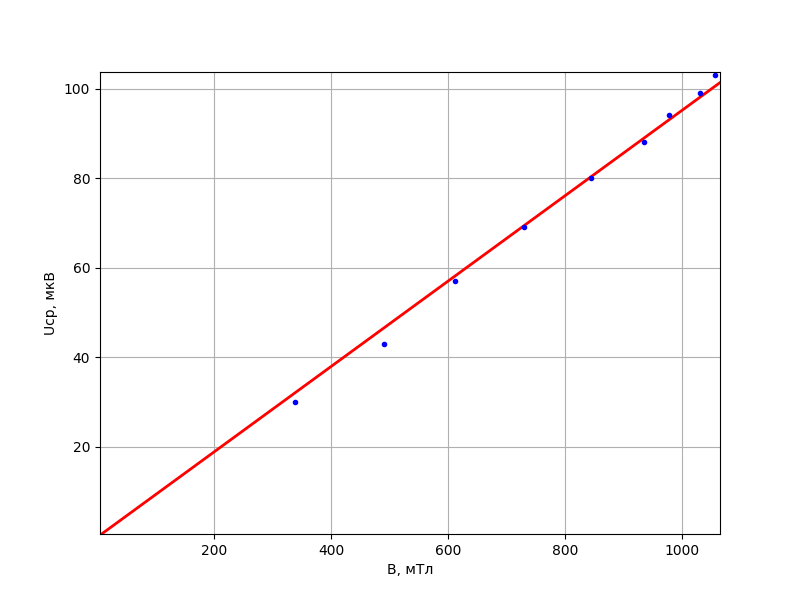
\includegraphics[scale=0.8]{Pictures/0,5мАмпер.png}
	\caption*{Рис. 5.}
\end{figure}

Из МНК:

$\mathscr{E}_X = k_2B$.

$k_2 = 9,53 \cdot 10^{-5} \text{ }\frac{\text{м}^2}{\text{c}}$;

$\sigma_{k_2} = 0,05\cdot 10^{-5} \text{ }\frac{\text{м}^2}{\text{c}}$.

Значит:

\vspace{2mm}

$n = \frac{I_0}{k_2ea} = 1,49\cdot 10^{16}$ см$^{-3}$; \hspace{42mm} $R_X = \frac{ak_2}{I_0} = 419\text{ }\frac{\text{см}^3}{\text{Кл}}$;

\vspace{2mm}
$\sigma_n = n\cdot \frac{\sigma_{k_2}}{k_2} = 0,01\cdot 10^{16}$ см$^{-3}$; \hspace{40mm} $\sigma_{R_X} = R_X \cdot \frac{\sigma_{k_2}}{k_2} = 2\text{ }\frac{\text{см}^3}{\text{Кл}}$;

\vspace{3mm}
$\boxed{n = (1,49 \pm 0,01)\cdot 10^{16} \text{ см}^{-3}} \hspace{38mm} \boxed{R_X = (419 \pm 2)\text{ }\frac{\text{см}^3}{\text{Кл}}}$

\vspace{7mm}
Найдем подвижность частиц $\mu$ из уравнения $\sigma = ne\mu$:

$\mu = \frac{\sigma}{ne} = 1,34\cdot 10^3$ $\frac{\text{см}^2}{\text{В}\cdot\text{с}}$

$\sigma_{\mu} = \mu \sqrt{\left(\frac{\sigma_{\sigma}}{\sigma}\right)^2 + \left(\frac{\sigma_n}{n}\right)^2} = 0,01\cdot 10^3$ $\frac{\text{см}^2}{\text{В}\cdot\text{с}}$

\vspace{3mm}
$\boxed{\mu = (1,34 \pm 0,01)\cdot 10^3 \text{ }\frac{\text{см}^2}{\text{В}\cdot\text{с}}}$



\vspace{7mm}
{\Large \textbf{3.}} $I_0 = 0,3$ мА, $U_0 = -10$ мкВ.

\begin{table}[h!]
	\centering
	\begin{tabular}{|c|c|c|c|c|c|}
		\hline
		\multirow{2}{*}{$I$, А} & \multirow{2}{*}{$B$, мТл} & \multirow{2}{*}{$+U_X$, мкВ} & \multirow{2}{*}{$-U_X$, мкВ} & \multicolumn{2}{c|}{$U_{\text{ср}}$}                   \\ \cline{5-6} 
		&                           &                              &                              & $\frac{(+U_X) - (-U_X)}{2}$, мкВ & $U_{34} - U_0$, мкВ \\ \hline
		2,0                     & 1057                      & 52                           & -72                          & 62                               & 62                  \\ \hline
		1,8                     & 1032                      & 50                           & -69                          & 60                               & 60                  \\ \hline
		1,6                     & 978                       & 47                           & -66                          & 57                               & 57                  \\ \hline
		1,4                     & 935                       & 44                           & -63                          & 54                               & 54                  \\ \hline
		1,2                     & 845                       & 39                           & -58                          & 49                               & 49                  \\ \hline
		1,0                     & 730                       & 32                           & -52                          & 42                               & 42                  \\ \hline
		0,8                     & 611                       & 24                           & -44                          & 35                               & 34                  \\ \hline
		0,6                     & 491                       & 17                           & -36                          & 27                               & 27                  \\ \hline
		0,4                     & 338                       & 8                            & -28                          & 18                               & 18                  \\ \hline
	\end{tabular}
	\caption*{Таблица 5}
\end{table}

И снова значения, полученные двумя способами, почти совпадают.

\newpage

Строим график $\mathscr{E}_X(B) = U_{\text{ср}}(B)$.

\begin{figure}[h!]
	\centering
	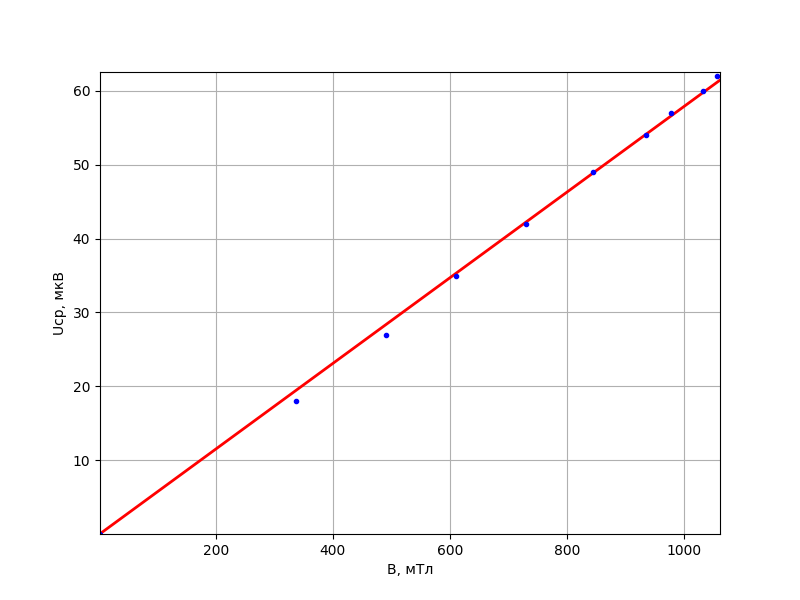
\includegraphics[scale=0.75]{Pictures/0,3мАмпер.png}
	\caption*{Рис. 6.}
\end{figure}

С помощью МНК получаем следующее:

$\mathscr{E}_X = k_3B$.

$k_3 = 5,80 \cdot 10^{-5} \text{ }\frac{\text{м}^2}{\text{c}}$;

$\sigma_{k_3} = 0,02\cdot 10^{-5} \text{ }\frac{\text{м}^2}{\text{c}}$.

Следовательно:

\vspace{2mm}

$n = \frac{I_0}{k_3ea} = 1,47\cdot 10^{16}$ см$^{-3}$; \hspace{42mm} $R_X = \frac{ak_3}{I_0} = 425\text{ }\frac{\text{см}^3}{\text{Кл}}$;

\vspace{2mm}
$\sigma_n = n\cdot \frac{\sigma_{k_3}}{k_3} = 0,01\cdot 10^{16}$ см$^{-3}$; \hspace{40mm} $\sigma_{R_X} = R_X \cdot \frac{\sigma_{k_3}}{k_3} = 2\text{ }\frac{\text{см}^3}{\text{Кл}}$;

\vspace{3mm}
$\boxed{n = (1,47 \pm 0,01)\cdot 10^{16} \text{ см}^{-3}} \hspace{38mm} \boxed{R_X = (425 \pm 2)\text{ }\frac{\text{см}^3}{\text{Кл}}}$

\vspace{7mm}
Найдем подвижность частиц $\mu$ из уравнения $\sigma = ne\mu$:

$\mu = \frac{\sigma}{ne} = 1,36\cdot 10^3$ $\frac{\text{см}^2}{\text{В}\cdot\text{с}}$

$\sigma_{\mu} = \mu \sqrt{\left(\frac{\sigma_{\sigma}}{\sigma}\right)^2 + \left(\frac{\sigma_n}{n}\right)^2} = 0,01\cdot 10^3$ $\frac{\text{см}^2}{\text{В}\cdot\text{с}}$

\vspace{3mm}
$\boxed{\mu = (1,36 \pm 0,01)\cdot 10^3 \text{ }\frac{\text{см}^2}{\text{В}\cdot\text{с}}}$

\begin{figure}[h!]
	\centering
	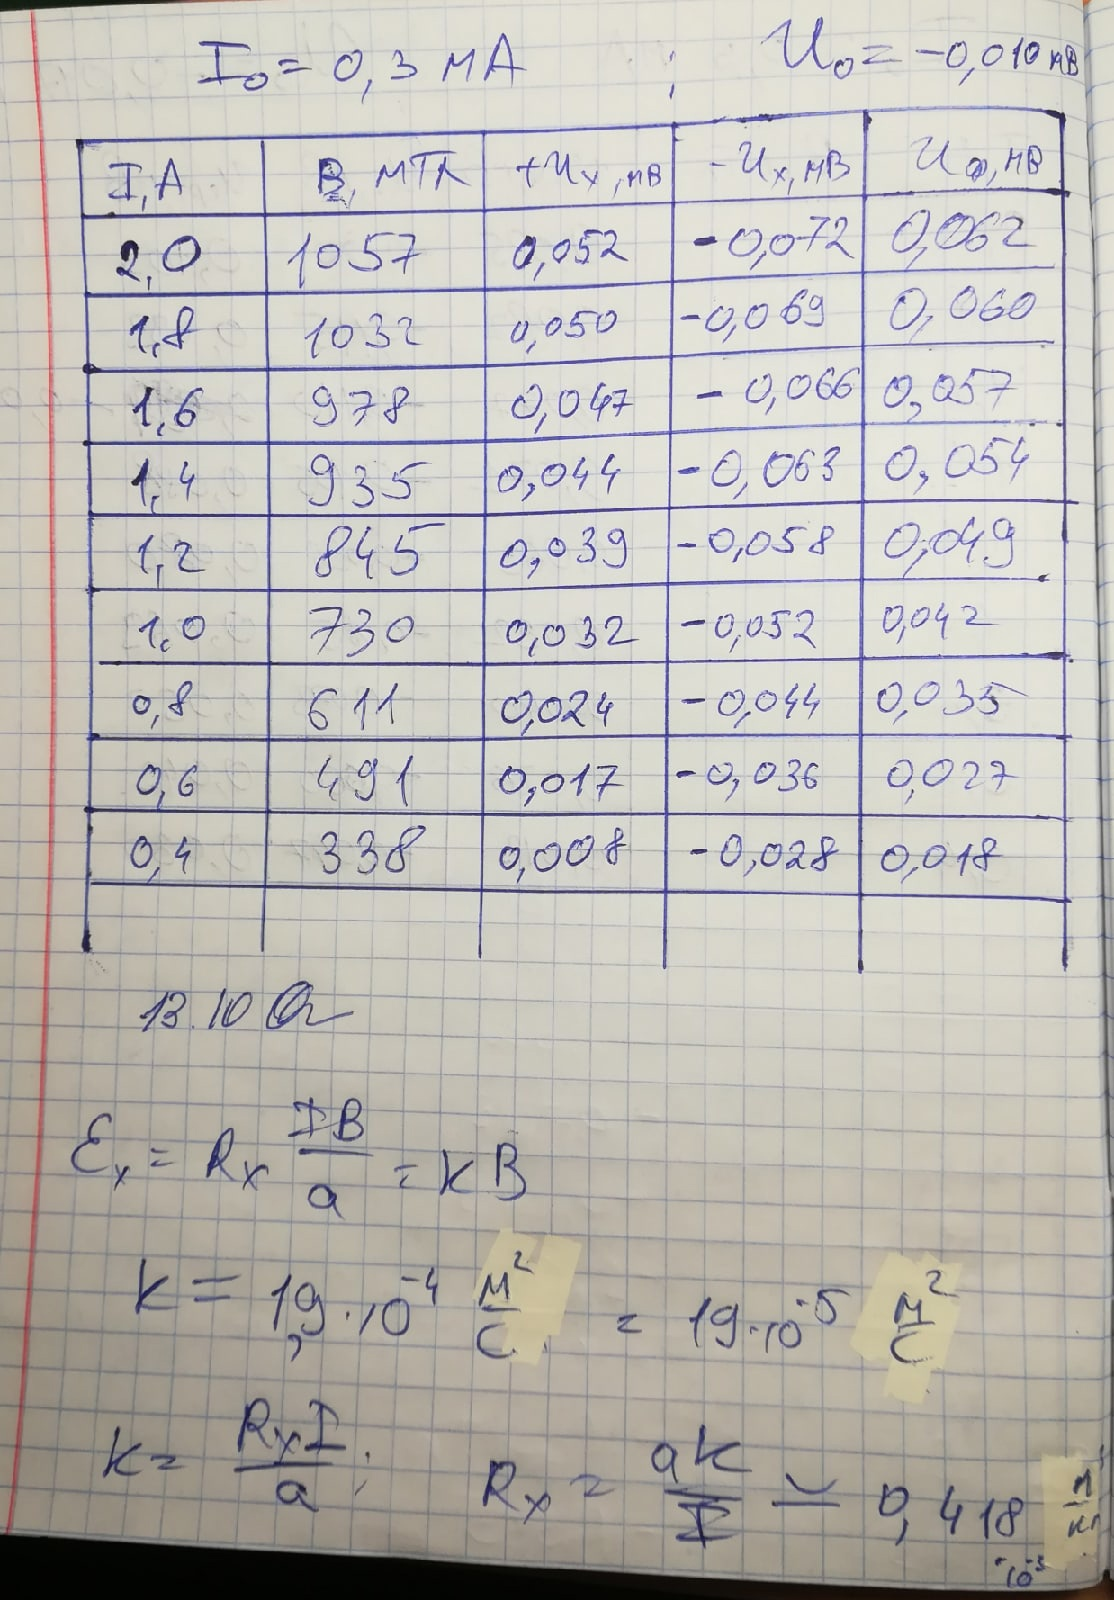
\includegraphics[scale=0.4]{Pictures/Подпись.jpg}
	\caption*{Рис. 7}
\end{figure}

Подытожим результат.

\begin{table}[h!]
	\centering
	\begin{tabular}{|c|c|c|c|}
		\hline
		$I_0$, мА & $n$, $10^{16}$ см$^{-3}$ & $R_X$,  $\frac{\text{см}^3}{\text{Кл}}$ & $\mu$, $10^3$ $\frac{\text{см}^2}{\text{В}\cdot\text{с}}$ \\ \hline
		1         & 1,51                     & 414                                     & 1,32                                                      \\ \hline
		0,5       & 1,49                     & 419                                     & 1,34                                                      \\ \hline
		0,3       & 1,47                     & 425                                     & 1,36                                                      \\ \hline
	\end{tabular}
	\caption*{Таблица 6}
\end{table}

Как видим, величины, соответствующие разным экспериментам, достаточно близки друг к другу.

$\overline{n} = 1,49 \cdot 10^{16}$ см$^{-3}$ \hspace{20mm} $\sigma_{\overline{n}} = \sqrt{\sigma_{n_1}^2 + \sigma_{n_2}^2 + \sigma_{n_3}^2} = 0,02\cdot 10^{16}$ см$^{-3}$;

\vspace{2mm}
$R_X = \overline{R_X} = 419$ $\frac{\text{см}^3}{\text{Кл}}$ \hspace{18mm} $\sigma_{R_X} = \sqrt{\sigma_{R_{X}^1}^2 + \sigma_{R_{X}^2}^2 + \sigma_{R_{X}^3}^2} = 4 \text{ }\frac{\text{см}^3}{\text{Кл}}$;

\vspace{2mm}
$\overline{\mu} = 1,34 \cdot 10^3$ $\frac{\text{см}^2}{\text{В}\cdot\text{c}}$ \hspace{23mm} $\sigma_{\overline{\mu}} = \sqrt{\sigma_{\mu_1}^2 + \sigma_{\mu_2}^2 + \sigma_{\mu_3}^2} = 0,02\text{ }\frac{\text{см}^2}{\text{В}\cdot\text{c}}$.
\vspace{85mm}

\textbf{{\large Вывод:}} в работе был исследован эффект Холла в полупроводнике, а именно в образце германия. Для него были найдены следующие параметры: 

1) удельное сопротивление $\rho_0 = (3120\pm 4)\cdot 10^{-4}\text{ Ом}\cdot\text{см}$;

2) удельная проводимость $\sigma = (3,200 \pm 0,004) \text{ } (\text{Ом}\cdot\text{см})^{-1}$;
	
3) концентрация носителей заряда $n = (1,49 \pm 0,02)\cdot 10^{16}\text{ см}^3$;

4) постоянна Холла $R_X = (419 \pm 4) \text{ }\frac{\text{см}^3}{\text{Кл}}$;

5) подвижность заряженных частиц $\mu = (1,34 \pm 0,02)\text{ }\frac{\text{см}^2}{\text{В}\cdot\text{c}}$.

\noindent Все ошибки связаны с неточностью измерений и несовершенством техники измерения.
\end{document}